\setAuthor{}
\setRound{lõppvoor}
\setYear{2020}
\setNumber{G 7}
\setDifficulty{7}
\setTopic{TODO}

\prob{Pulgad}
\begin{wrapfigure}{r}{0.35\textwidth}
  \vspace{-8pt}
  \begin{center}
  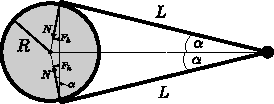
\includegraphics[scale=0.9]{2020-v3g-07-yl.pdf}
  \end{center}
  \vspace{-25pt}
\end{wrapfigure}
Kaks pulka pikkusega $L$ on otsapidi kinnitatud hõõrdevaba kinnitusega.
Hõõrdevabal horisontaalsel laual on silinder raadiusega $R$ ja massiga $m$.
Joonisel on kujutatud silinder ja pulgad pealtvaates. Eeldame, et pulki hoitakse
alati horisontaalselt nagu joonisel, nendega haaratakse kinni silindri keskelt,
pulkade otsad on täpselt silindri puutepunktides ning pulkade mass on tühine.
Samuti eeldame, et silindri massikese on puutepunkte ühendava lõigu keskpunktis.\\
\osa Leidke minimaalne hõõrdetegur $\mu_{\min}$ pulkade ja silindri vahel,
et silindrist pulkade abil kinni haarates see pulkade vahelt ära ei libiseks.\\
\osa Olgu hõõrdetegur pulkade ja silindri vahel $\mu > \mu_{\min}$. Leidke
minimaalne vajalik jõumoment $\tau_{\min}$, mida tuleb pulkadele avaldada, et
silindrist pulkade abil kinni haarates oleks võimalik silinder laualt üles
tõsta. Maa raskuskiirendus on $g$.


\hint

\solu
\osa Olgu silindrile mõjuv normaaljõud kummaski punktis $N$ (puutujaga risti) ning hõõrdejõud $F_h$ (puutujaga paralleelne). Olgu nurk pulkade vahel $2\alpha$.

\begin{figure}[h]
\centering
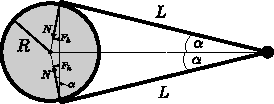
\includegraphics[width=0.5\linewidth]{2020-v3g-07-sol.pdf}
\end{figure}

Jõudude tasakaalust saame, et puutepunktides mõjuvad resultantjõud $\vec N + \vec{F_h}$ peavad olema paralleelsed ja vastassuunalised, seega sümmeetria tõttu peab $\vec N + \vec{F_h}$ olema sümmeetriateljega risti.

Kuna puutuja on raadiusega risti, on lihtne näidata, et nurk $\vec N$ ja puutepunkte ühendava sirge vahel on $\alpha$, seega $\tan \alpha = \frac{F_h}{N}$. Piirjuhul, kus $\mu$ on minimaalne, $F_h = \mu N$ ja seega
$$\tan \alpha = \frac{\mu N}{N} = \mu$$

Teisalt $\tan \alpha = \frac{R}{L}$, seega
$$\mu_\text{min} = \frac{R}{L}$$

\osa Nagu eelmises osas näidatud, siis hõõrdejõu lauaga paralleelne komponent $F_{h,r} = N\tan \alpha = \frac{R}{L}\cdot N$. Silindrit üles tõstes peab raskusjõu tasakaalustamiseks lisaks mõjuma kummaski punktis hõõrdejõu lauaga risti olev komponent $F_{h,t} = \frac{mg}{2}$, seega kui summaarne hõõrdejõud on $F_h$, siis
$$F_h^2 = F_{h,r}^2 + F_{h,t}^2 = \frac{R^2}{L^2}N^2 + \frac{m^2g^2}{4}$$

Piirjuhul $F_h = \mu N$ ja $\tau = NL$, seega
$$\mu^2N^2 = \frac{R^2}{L^2}N^2 + \frac{m^2g^2}{4}$$
$$\left(\mu^2 - \frac{R^2}{L^2}\right)N^2 = \frac{m^2g^2}{4}$$
$$N = \frac{mg}{2\sqrt{\mu^2-\frac{R^2}{L^2}}}$$
$$\tau_\text{min} = NL = \frac{mgL}{2\sqrt{\mu^2-\frac{R^2}{L^2}}} = \frac{mgL^2}{2\sqrt{L^2\mu^2 - R^2}}$$
\probend